\newcommand{\env}[1]{\texttt{#1}}
\newcommand{\command}[1]{\texttt{#1}}
\newcommand{\package}[1]{\texttt{\itshape#1}}
\newcommand{\engl}[1]{(engl: \textit{#1})\xspace}
\setlength{\parindent}{0pt}
\lstset{extendedchars=\true}
\lstset{inputencoding=ansinew}
\newcommand\tab[1][1cm]{\hspace*{#1}}
\newpage

\section{Aufgabe}

\subsection{Frage- bzw. Aufgabenstellung}

Sie erhalten in dieser Woche die Gelegenheit, den bisher im Modul behandelten Stoff zu vertiefen.
Die folgende Praktikumsaufgabe soll Ihnen dabei helfen. \\
\\
Arbeiten Sie die bisher bereitgestellten Vorlesungsmaterialien nochmals nach. Fangen Sie dort
an, wo Sie meinen, den größten Nachholbedarf zu haben, bzw. dort, wo Sie unsicher sind ob
Sie alles verstanden haben.

\subsection{Teilaufgabe 1}

\subsubsection{Frage- bzw. Aufgabenstellung}
Beschreiben Sie mit eigenen Worten und einer Skizze, wie Browser-Cookies funktionieren!

\subsubsection{Lösung}\cite{[1]}
Cookies sind Informationen die von einer besuchten Website auf dem eigenen Computer abgelegt werden, damit zum Beispiel Daten aus einem Warenkorb in einem Online-Shop nicht verloren gehen wenn man die Seite schließt und wieder öffnet. Dies ist nötig, da HTTP ein zustandsloses Protokoll ist und die Seitenaufrufe so unabhängig voneinander sind. Die Funktionsweise der Cookies ist ziemlich simpel. Der Webserver setzt bei Antworten im Browser einen Cookie. Dies wird über eine zusätzliche Cookie-Zeile geregelt, wodurch der Webserver den User wiedererkennen kann. Der einfachste Aufbau eines Cookies besteht aus einem Namen und einem Wert, was dann in etwa so aussehen könnte: \\
\\
\textit{Set-Cookie: TestCookie = 1236326} \\
\\
Diese Skizze veranschaulicht die Kommunikation zwischen dem User und dem Server: 

\begin{figure}[htbp]
\begin{center}
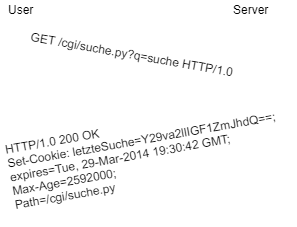
\includegraphics[width=0.5\textwidth]{Bild3}
\caption{Beispielskizze zu Browser-Cookies}
\end{center}
\end{figure}


\subsubsection{Ergebnis}
Wir wissen was Browser-Cookies sind und können diese mithilfe einer Skizze veranschaulichen.

\subsection{Teilaufgabe 2}

\subsubsection{Frage- bzw. Aufgabenstellung}
Formulieren Sie mindestens fünf Kurzfragen, die in Stichworten zu beantworten sind. Die Aufgaben sollen im Stil von Klausurfragen gestellt werden. Gerne dürfen Sie eine eigene Aufgabe zur UDP Prüfsumme und der Nummerierung von TCP Paketen mit Sequenz- und ACK-Nr. entwerfen und lösen. Zur Ideenfindung beachten Sie auch den Artikel zum Thema Internet Peering, der Stoff aus Vorlesung Nr.2 wiederholt und vertieft.

\subsubsection{Lösung}
1. Welche Kommunikationsformen gibt es und wie funktionieren sie? \\
\\
- \textit{Client-Server-Modell}: ein Host (Client) ruft Informationen von einem anderen Host (Server) ab \\
- \textit{Peer-to-Peer-Modell}: gleichgestellte Hosts (Peers) tauschen gegenseitig Informationen aus \\
\\
2. Was ist \textit{MPEG-DASH} und wie funktioniert es? \\
\\
- \textit{Server}: Unterteilt das Video in Chunks, wobei jeder Chunk mit unterschiedlichen Bitraten abgespeichert wird. Eine sogenannte \textit{Manifest-Datei} enthält die URLs für die Chunks. \\
\\
- \textit{Client}: Misst während des Abspielens die Bandbreite zwischen Client und Server. In der Manifest-Datei wird geguckt welcher Chunk gewählt werden sollte, wobei die maximal mögliche Bitrate gemäß der aktuellen Bandbreite der Verbindung ausgewählt wird. \\
\\
3. Wie sieht der Protokollstapel des Internets aus? \\
\\
- (von oben nach unten): Anwendung, Transport, Netzwerk, Sicherung, Bitübertragung \\
\\
4. Addieren Sie diese zwei 16-Bit-Integer-Werte (1011001110110110,1001101110101100) und erstellen Sie die Prüfsumme. 
\begin{table}[htbp]
\centering
\caption{Prüfsummenbeispiel}
\label{my-label}
\begin{tabular}{ll}
Zahl 1    & 1011001110110110  \\
Zahl 2    & 1001101110101100  \\
Übertrag  & 10100111101100010 \\
Summe     & 0100111101100011  \\
Prüfsumme & 1011000010011100 
\end{tabular}
\end{table}

5. Warum ist TCP fair? \\
\\
Wenn zwei Verbindungen im Wettbewerb sind führt \textit{Additive Increase} zu einer Steigerung von 1, wenn der Durchsatz wächst während \textit{Multiplicative Decrease} den Durchsatz proportional reduziert.

\subsection{Teilaufgabe 3}

\subsubsection{Frage- bzw. Aufgabenstellung}
Entwickeln Sie eine kurze Programmieraufgabe (Frage und Lösung dazu). Diese Aufgabe soll einen Teilbereich Ihrer Wahl aus dem bisher behandelten Vorlesungsstoff abdecken.

\subsubsection{Lösung}

\textbf{Aufgabe}: \\
\\ 
Erstellen Sie in Java einen Clienten der mithilfe der OpenWeatherMap die aktuelle Temperatur und Wetterlage (wolkig, sonnig etc) einer Stadt ausgeben kann. Übergeben Sie hierfür die Postleitzahl und den Ländercode (jedoch soll auch er Stadtname ausgegeben werden). Wie die Daten entgegen genommen werden bleibt ihnen überlassen (XML oder JSON).  \\
\\
\textbf{Lösung}: \\
\\
Für die Lösung dieser Aufgabe wurde eine Klasse mit dem Namen \textit{CurrentTemp} erstellt in der alle Methoden, inklusive der main-Methode, realisiert wurden. \\
\\
Zunächst wurde eine \textit{readUrl}-Methode geschrieben, der man eine URL-Adresse übergibt und alle Zeichen auf dieser Seite einem StringBuilder hinzufügt und diesen dann auch zurückgibt (siehe Zeile 1 bis 16).

\begin{lstlisting}[caption={readUrl-Methode}]
private static String readUrl(String urlString) throws Exception {

	BufferedReader reader = null;
	try {
		URL url = new URL(urlString);
		reader = new BufferedReader(new InputStreamReader(url.openStream()));
		StringBuilder sb = new StringBuilder();
		int read;
		while ((read = reader.read()) != -1)
			sb.append((char) read);
		return sb.toString();
	} finally {
		if (reader != null)
			reader.close();
	}
}
\end{lstlisting}

Da die Daten im JSON-Format immer in einer untergeordneten Sammlung über Name/Werte-Paare gespeichert sind, muss man zunächst gucken wie man an die Daten der API kommt. Dazu eignet sich die Seite \url{https://jsonformatter.curiousconcept.com/} (aus dem letzten Praktikum). Hier werden die JSON-Daten vernünftig formatiert, so dass man einen guten Überblick über alle Daten bekommt. Wie man in Abbildung 1 sieht, sind die Daten für die Temperatur in einem \textit{main}-Objekt zu finden. Die Stadt befindet sich ganz unten in einem \textit{name} String und die Wetterlage ist in dem Array \textit{weather} zu finden.

\begin{figure}[htbp]
\begin{center}
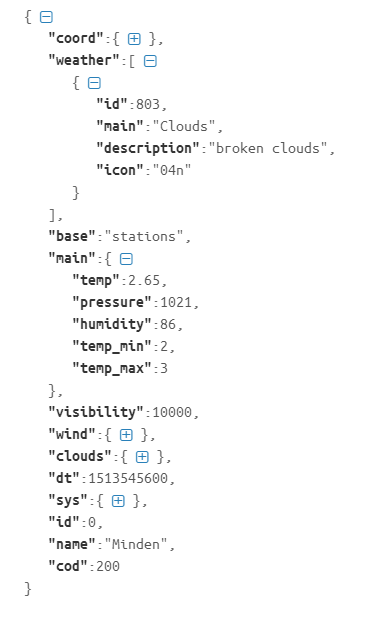
\includegraphics[width=0.5\textwidth]{Bild1}
\caption{Formatierte JSON-Datei der API}
\end{center}
\end{figure}

Die zweite Methode namens \textit{ausgabeTemp} übernimmt den wichtigsten Teil der Aufgabe, da sie dafür sorgt, dass wir am Ende die Ausgabe des Wetters auf der Konsole haben. Da wir hier mit dem JSON-Format arbeiten, benutzen wir das \textit{org.json}-package, um mit den JSON-Objekten zu arbeiten. \\
\\
Zu Beginn wird der \textit{Scanner} benutzt, damit der Benutzer die Postleitzahl, so wie den Ländercode eingeben kann. Anschließend wird ein neues JSONObject erstellt, dem man dann mithilfe der \textit{readUrl}-Methode die API der OpenWeatherMap zusammen mit der zuvor eingegebenen Postleitzahl (plus zugehörigem Ländercode) übergibt (siehe Zeile 1 bis 9). Wichtig für die URL ist auch der Parameter \textit{units=metric}, damit die Angaben in Celsius erfolgen und nicht in Fahrenheit. Außerdem wäre es sinnvoll den API-Key vom Praktikumsblatt anzugeben. Dazu benutzt man den Parameter \textit{APPID}\\
\\


In Zeile 9 bis 15 greifen wir dann auf die verschiedenen Objekte der JSON-Datei zu, die wir für diese Aufgabe brauchen. Dies wären dann die jetzige Temperatur über das Objekt \textit{main} (Zeile 13,14), der Stadtname (Zeile 15) und die Wetterlage über das Array \textit{weather} und den String \textit{main} (Zeile 10 bis 12). Anschließend geben wir alle notwendigen Daten aus. \\

\begin{lstlisting}[caption={ausgabeTemp}]
private static void ausgabeTemp() throws Exception {
	Scanner scan = new Scanner(System.in);
	System.out.println("Geben Sie bitte die Postleitzahl ein: ");
	String zipCode = scan.nextLine();
	System.out.println("Geben Sie bitte den Ländercode ein: ");
	String countryCode = scan.nextLine();
	scan.close();
	try {
		JSONObject json = new JSONObject(readUrl("http://api.openweathermap.org/data/ 2.5/weather?zip="+zipCode+","+countryCode+"&units=metric
		&APPID=722920868a0a0266c859a174da690bc1"));
		JSONArray weatherArray = json.getJSONArray("weather");
		JSONObject weatherObject = weatherArray.getJSONObject(0);
		String weatherCurrent = weatherObject.getString("main");
		JSONObject main = json.getJSONObject("main");
		int temp = main.getInt("temp");
		String cityName = json.getString("name");
		System.out.println(zipCode + ", "+ cityName + ": " + temp + "°C, " + weatherCurrent);
	} catch (JSONException e) {
		System.out.println("Stadt nicht gefunden");
		e.printStackTrace();
	}
}
\end{lstlisting}

In der main steht schließlich nur noch die statische Methode \textit{ausgabeTemp}.

\begin{lstlisting}[caption={main}]
public static void main(String[] args) throws Exception {
		ausgabeTemp();
}
\end{lstlisting}

\newpage

Die Ausgabe könnten dann so aussehen: 

\begin{figure}[htbp]
\begin{center}
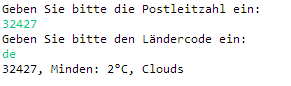
\includegraphics[width=0.6\textwidth]{Bild2}
\caption{aktuelles Wetter, Minden}
\end{center}
\end{figure}


\subsubsection{Ergebnis}

Wir können mithilfe der OpenWeatherMap das aktuelle Wetter einer Stadt anzeigen lassen.

\section{Quellen}
\begin{thebibliography}{999}
\bibitem {1} Agnieszka Czernik, Cookies – Funktion und Aufbau einfach erklärt \\ \url{www.datenschutzbeauftragter-info.de/cookies-funktion-und-aufbau-einfach-erklaert/}, 17.12.2017

\end{thebibliography}







